\section{Koordinatensysteme}
\subsection{2D Koordinatensysteme}
\subsubsection{Kartesische Koordinaten}
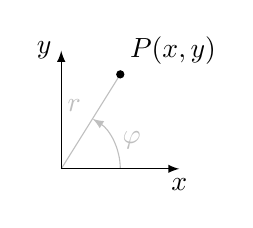
\begin{tikzpicture} [baseline=(current bounding box.north), scale = 1.5]
    % Winkel phi
    \draw [lightgray, -{latex}] (0.5, 0) arc (0:58:0.5) node [text=lightgray, midway, right] {$\varphi$};

    % Länge r
    \draw [lightgray] (0, 0) -- (0.5, 0.8) node [text=lightgray, midway, above left] {$r$};

    % Kartesische Achsen
    \draw[{latex}-{latex}] (0, 1) node [left]  {$y$} --  (0, 0) -- (1, 0) node [below] {$x$} ;
    % \draw[-{latex}] (0, 0) --  ;
    
    % Punkt p
    \fill (0.5, 0.8) circle (1pt) node [anchor=south west] {$P(x,y)$};
\end{tikzpicture}\hfill
\begin{minipage}[t]{.8\columnwidth}
    \centering
    \myul{Polar \textrightarrow\ Kartesisch}
    \[
    \begin{pmatrix}
        x \\
        y
    \end{pmatrix}
    =
    \begin{pmatrix}
        r \cdot \cos{\varphi}\\
        r \cdot \sin{\varphi}
    \end{pmatrix}
    \]
\end{minipage}


\subsubsection{Polarkoordinaten}
\begin{tikzpicture} [baseline=(current bounding box.north), scale = 1.5]
    % Kartesische Achsen
    \draw (0, 0) -- ($(0.5,0)+(.13333pt,0)$);
    \draw[lightgray, -{latex[lightgray]}]($(0.5,0)+(.13333pt,0)$) -- (1, 0) node [text=lightgray, below] {$x$} ;
    \draw[lightgray, -{latex}] (0, 0) -- (0, 1) node [text=lightgray, left]  {$y$} ;

    % Punkt p
    \fill (0.5, 0.8) circle (1pt) node [anchor=south west] {$P(r,\varphi)$};

    % Länge r
    \draw (0, 0) -- (0.5, 0.8) node [midway, above left] {$r$};
    % Winkel phi
    \draw [-{latex}] (0.5, 0) arc (0:58:0.5) node [midway, right] {$\varphi$};
\end{tikzpicture}\hfill
\begin{minipage}[t]{.8\columnwidth}
    \centering
    \myul{Kartesisch \textrightarrow\ Polar}
    \[
    \begin{pmatrix}
        r \\
        \varphi
    \end{pmatrix}
    =
    \begin{pmatrix}
        \sqrt{x^2+y^2}\\
        \tan^{-1}{\frac{y}{x}}
    \end{pmatrix}
    \]
\end{minipage}


\subsection{3D Koordinatensysteme}
\subsubsection{Kartesische Koordinaten}
\tdplotsetmaincoords{70}{110}
\begin{tikzpicture}[baseline=(current bounding box.north), tdplot_main_coords, scale=2]
    % Koordinatensystem
    \draw [-{latex}] (0, 0, 0) -- (1, 0, 0) node [below left] {$x$};
    \draw [-{latex}] (0, 0, 0) -- (0, 1, 0) node [right]      {$y$};
    \draw [-{latex}] (0, 0, 0) -- (0, 0, 1) node [right]      {$z$};
    % Punkt bei (0.75,0.75,0.75)
    \fill (0.75, 0.75, 0.75) circle (1pt) node [above right] {$P(x, y, z)$};
    % Koordinatenkomponenten
    \draw [dashed] (0, 0.75, 0)    -- (0.75, 0.75, 0)    node [midway, below right] {$x$};
    \draw [dashed] (0.75, 0, 0)    -- (0.75, 0.75, 0)    node [midway, below left]  {$y$};
    \draw [dashed] (0.75, 0.75, 0) -- (0.75, 0.75, 0.75) node [midway, right]       {$z$};
\end{tikzpicture}\hfill
\begin{minipage}[t]{.6\columnwidth}
    \centering
    \myul{Zylindrisch \textrightarrow\ Kartesisch}
    \[
    \begin{pmatrix}
        x \\
        y \\
        z
    \end{pmatrix}
    =
    \begin{pmatrix}
        r \cdot \cos{\varphi}\\
        r \cdot \sin{\varphi}\\
        z
    \end{pmatrix}
    \]

    \myul{Sphärisch \textrightarrow\ Kartesisch}
    \[
    \begin{pmatrix}
        x \\
        y \\
        z
    \end{pmatrix}
    =
    \begin{pmatrix}
        r \cdot \sin{\theta} \cdot \cos{\varphi}\\
        r \cdot \sin{\theta} \cdot \sin{\varphi}\\
        r \cdot \cos{\theta}
    \end{pmatrix}
    \]
\end{minipage}


\subsubsection{Zylinderkoordinaten}
\tdplotsetmaincoords{70}{110}
\begin{tikzpicture}[baseline=(current bounding box.north), tdplot_main_coords, scale=2]
    % Koordinatensystem
    \draw [-{latex}] (0, 0, 0) -- (1, 0, 0) node [below left] {$x$};
    \draw [-{latex}] (0, 0, 0) -- (0, 1, 0) node [right]      {$y$};
    \draw [-{latex}] (0, 0, 0) -- (0, 0, 1) node [right]      {$z$};
    % Punkt bei (0.75,0.75,0.75)
    \fill (0.75, 0.75, 0.75) circle (1pt) node [above right] {$P(r_{\rm z}, \varphi, z)$};
    % Koordinatenkomponenten
    \draw [dashed] (0,0,0)         --  (0.75, 0.75, 0)    node [midway, above right] {$r_{\rm z}$};
    \draw [-{latex}]     (0.5,0,0)       arc (0:45:0.5)         node [midway, below]       {$\varphi$};
    \draw [dashed] (0.75, 0.75, 0) --  (0.75, 0.75, 0.75) node [midway, right]       {$z$};
\end{tikzpicture}\hfill
\begin{minipage}[t]{.6\columnwidth}
    \centering
    \myul{Kartesisch \textrightarrow\ Zylindrisch}
    \[
    \begin{pmatrix}
        r \\
        \varphi \\
        z
    \end{pmatrix}
    =
    \begin{pmatrix}
        \sqrt{x^2+y^2}\\
        \tan^{-1}{\frac{y}{x}}\\
        z
    \end{pmatrix}
    \]

    \myul{Sphärisch \textrightarrow\ Zylindrisch}
    \[
    \begin{pmatrix}
        r_{\rm z} \\
        \varphi \\
        z
    \end{pmatrix}
    =
    \begin{pmatrix}
        r_{\rm s} \cdot \sin{\theta}\\
        \phi\\
        r_{\rm s} \cdot \cos{\theta}
    \end{pmatrix}
    \]
\end{minipage}


\subsubsection{Kugelkoordinaten / Sphärische Koordinaten}
\tdplotsetmaincoords{70}{110}
\begin{tikzpicture}[baseline=(current bounding box.north), tdplot_main_coords, scale=2]
    % Koordinatensystem
    \draw [-{latex}] (0, 0, 0) -- (1, 0, 0) node [below left] {$x$};
    \draw [-{latex}] (0, 0, 0) -- (0, 1, 0) node [right]      {$y$};
    \draw [-{latex}] (0, 0, 0) -- (0, 0, 1) node [right]      {$z$};
    % Punkt bei (0.75,0.75,0.75)
    \fill (0.75, 0.75, 0.75) circle (1pt) node [above right] {$P(r_{\rm s}, \theta, \phi)$};
    % Koordinatenkomponenten
    \draw [dotted] (0,0,0) -- (0.75, 0.75, 0) -- (0.75, 0.75, 0.75);
    \draw [-{latex}]     (0.5,0,0) arc (0:45:0.5)         node [midway, below]       {$\phi$};
    \draw [dashed] (0, 0, 0) --  (0.75, 0.75, 0.75) node [midway, below right] {$r_{\rm s}$};
    \tdplotsetthetaplanecoords {90}
    \tdplotdrawarc [tdplot_rotated_coords, -{latex}] {(0, 0, 0)} {0.5} {0} {45} {anchor=south} {$\theta$}
\end{tikzpicture}
% \subsection{Kartesische Koordinaten}
% \subsubsection{2D}




% \subsubsection{3D}



% \subsection{Polarkoordinaten}



% \subsection{Zylinderkoordinaten}



% \subsection{Sphärische Koordinaten / Kugelkoordinaten}



% \section{Integration}

% \subsection{Umrechnungen}
% \subsubsection{Kartesische Koordinaten $\leftrightarrow$ Polarkoordinaten}



% \subsection{Anwendungsformeln}
% \resizebox{\linewidth}{!}{
%     \begin{tabular}{|l|l|l|}
%         \hline
%         \bf{Allgemein} & \bf{Kartesische Koordinaten} & \bf{Polarkoordinaten} \\
%         \hline

%         \multicolumn{3}{|l|}{\bf{Flächeninhalt einer ebenen Figur $F$}} \\\hline
%         $ A = \iint\limits_{F} \diff a $ & 
%         $ = \int\limits_{X}\int\limits_{Y} \diff y \diff x $ &
%         $ = \int\limits_{\Phi}\int\limits_{R} r \diff r \diff \varphi $ \\\hline

%         \multicolumn{3}{|l|}{\bf{Oberfläche einer Ebene in drei Dimensionen}} \\\hline
%         % TODO: Evtl. umschreiben, dass man es besser versteht...
%         $ S = \iint\limits_{A} \frac{1}{\cos \gamma} \diff a $ & 
%         $ = \int\limits_{X}\int\limits_{Y} \sqrt{1 + \left(\frac{\partial z}{\partial x}\right)^2 + \left(\frac{\partial z}{\partial y}\right)^2} \diff y \diff x $ &
%         $ = \int\limits_{\Phi}\int\limits_{R} \sqrt{r^2 + r^2\left(\frac{\partial z}{\partial r}\right)^2 + \left(\frac{\partial z}{\partial \varphi}\right)^2} \diff r \diff \varphi $ \\\hline
        
%         \multicolumn{3}{|l|}{\bf{Volumen eines Zylinders}} \\\hline
%         $ V = \iint\limits_{A} z \diff a $ & 
%         $ = \int\limits_{X}\int\limits_{Y} z \diff y \diff x $ &
%         $ = \int\limits_{\Phi}\int\limits_{R} z r \diff r \diff \varphi $ \\\hline

%         \multicolumn{3}{|l|}{\bf{Trägheitsmoment einer ebenen Figur $F$, bezogen auf die x-Achse}} \\\hline
%         $ I_x = \iint\limits_{F} y^2 \diff a $ & 
%         $ = \int\limits_{X}\int\limits_{Y} (y^2) \diff y \diff x $ &
%         $ = \int\limits_{\Phi}\int\limits_{R} (r^2 \sin^2\varphi) r \diff r \diff \varphi $ \\\hline

%         \multicolumn{3}{|l|}{\bf{Trägheitsmoment einer ebenen Figur $F$, bezogen auf den Pol $(0, 0)$}} \\\hline
%         $ I_x = \iint\limits_{F} r^2 \diff a $ & 
%         $ = \int\limits_{X}\int\limits_{Y} (x^2 + y^2) \diff y \diff x $ &
%         $ = \int\limits_{\Phi}\int\limits_{R} (r^2) r \diff r \diff \varphi $ \\\hline

%         \multicolumn{3}{|l|}{\bf{Masse einer ebenen Figur $F$ mit Dichtefunktion $\varrho$}} \\\hline
%         $ m = \iint\limits_{F} \varrho \diff a $ & 
%         $ = \int\limits_{X}\int\limits_{Y} \varrho (x, y) \diff y \diff x $ &
%         $ = \int\limits_{\Phi}\int\limits_{R} \varrho (r, \varphi) r \diff r \diff \varphi $ \\\hline

%         \multicolumn{3}{|l|}{\bf{Koordinaten des Schwerpunkts $S$ einer homogenen, ebenen Figur $F$}} \\\hline
%         $ x_{S} = \frac{\iint\limits_{F} x \diff a}{A} $ & 
%         $ = \frac{\int\limits_{X}\int\limits_{Y} x \diff y \diff x}{\int\limits_{X}\int\limits_{Y} \diff y \diff x} $ &
%         $ = \frac{\int\limits_{\Phi}\int\limits_{R} r^2 \cos \varphi \diff r \diff \varphi}{\int\limits_{\Phi}\int\limits_{R} r \diff r \diff \varphi} $ \\
%         $ y_{S} = \frac{\iint\limits_{F} y \diff a}{A} $ & 
%         $ = \frac{\int\limits_{X}\int\limits_{Y} y \diff y \diff x}{\int\limits_{X}\int\limits_{Y} \diff y \diff x} $ &
%         $ = \frac{\int\limits_{\Phi}\int\limits_{R} r^2 \sin \varphi \diff r \diff \varphi}{\int\limits_{\Phi}\int\limits_{R} r \diff r \diff \varphi} $ \\\hline
%     \end{tabular}
% }

% \resizebox{\linewidth}{!}{
%     \begin{tabular}{|l|l|l|l|}  
%         \hline
%         \bf{Allgemein} & \bf{Kartesische Koordinaten} & \bf{Zylinderkoordinaten} & \bf{Kugelkoordinaten} \\
%         \hline
%         \multicolumn{4}{|l|}{\bf{Volumen eines Körpers $K$}} \\
%         \hline
%         $ V = \iiint\limits_{K} \diff V $ & 
%         $ = \iiint \diff x \diff y \diff z $ &
%         $ = \iiint r \diff r \diff \phi \diff z $ &
%         $ = \iiint r^2 \sin \theta \diff \theta \diff \phi \diff r $ \\
%         \hline

%         \multicolumn{4}{|l|}{\bf{Trägheitsmoment eines Körpers $K$, bezogen auf die Z-Achse}} \\
%         \hline
%         $ I_z = \iiint\limits_{K} r^2 \diff V $ & 
%         $ = \iiint (x^2 + y^2) \diff x \diff y \diff z $ &
%         $ = \iiint (r^2) r \diff r \diff \phi \diff z $ &
%         $ = \iiint (r^2 \sin^2 \theta) r^2 sin \theta \diff \theta \diff \phi \diff r $ \\
%         \hline

%         \multicolumn{4}{|l|}{\bf{Masse eines Körpers $K$ mit der Dichtefunktion $\varrho$}} \\
%         \hline
%         $ M = \iiint\limits_{K} \varrho \diff V $ & 
%         $ = \iiint \varrho (x, y, z) \diff x \diff y \diff z $ &
%         $ = \iiint \varrho (r, \phi, z) r \diff r \diff \phi \diff z $ &
%         $ = \iiint \varrho (r, \theta, \phi) r^2 sin \theta \diff \theta \diff \phi \diff r $ \\
%         \hline

%         \multicolumn{4}{|l|}{\bf{Koordinaten des Schwerpunktes $S$ eines homogenen Körpers $K$}} \\
%         \hline
%         $ x_{S} = \frac{\iiint\limits_{K} x \diff V}{V} $ & 
%         $ = \frac{\iiint (x) \diff x \diff y \diff z}{V} $ &
%         $ = \frac{\iiint (r \cos \phi) r \diff r \diff \phi \diff z}{V} $ &
%         $ = \frac{\iiint (r \sin \theta \cos \phi) r^2 sin \theta \diff \theta \diff \phi \diff r}{V} $ \\

%         $ y_{S} = \frac{\iiint\limits_{K} y \diff V}{V} $ & 
%         $ = \frac{\iiint (y) \diff x \diff y \diff z}{V} $ &
%         $ = \frac{\iiint (r \sin \phi) r \diff r \diff \phi \diff z}{V} $ &
%         $ = \frac{\iiint (r \sin \theta \sin \phi) r^2 sin \theta \diff \theta \diff \phi \diff r}{V} $ \\

%         $ z_{S} = \frac{\iiint\limits_{K} z \diff V}{V} $ & 
%         $ = \frac{\iiint (z) \diff x \diff y \diff z}{V} $ &
%         $ = \frac{\iiint (z) r \diff r \diff \phi \diff z}{V} $ &
%         $ = \frac{\iiint (r \cos \theta) r^2 sin \theta \diff \theta \diff \phi \diff r}{V} $ \\
%         \hline
%     \end{tabular}
% }